\documentclass[11pt,a4paper]{article}

\usepackage[margin=1in]{geometry}
\usepackage[T1]{fontenc}
\usepackage[utf8]{inputenc}
\usepackage{lmodern}
\usepackage{microtype}
\usepackage{amsmath, amssymb, amsfonts}
\usepackage{booktabs}
\usepackage{longtable}
\usepackage{array}
\usepackage{multirow}
\usepackage{xcolor}
\usepackage{hyperref}
\usepackage{enumitem}
\usepackage{graphicx}
\usepackage{float}
\usepackage{tikz}
\usepackage{pgfplots}
\pgfplotsset{compat=1.18}
\usetikzlibrary{arrows.meta, positioning, shapes.geometric, fit, backgrounds, matrix}

\hypersetup{
  colorlinks=true,
  linkcolor=blue!60!black,
  urlcolor=blue!60!black,
  citecolor=blue!60!black,
  pdftitle={Context-Aware Stance Detection Model Report},
  pdfauthor={OpenAI Codex}
}

\title{Graph-Statistic-Aware and Ancestor-Context-Aware Stance Detection for Syncialo\\
\large A Research-Oriented Technical Report on Architecture, Features, Training, Ablations, and Evaluation}
\author{Technical research report}
\date{\today}

\begin{document}
\maketitle

\begin{abstract}
This document presents a research-style analysis of two structured stance detection models for directed relation classification in debate graphs: an earlier graph-statistic-aware model and a later graph-ancestor-context-aware model. The task is to classify each candidate edge between two claims as \texttt{support}, \texttt{attack}, or \texttt{neutral}. Both models retain the same two pretrained text-pair subsystems, namely a natural language inference model and a target-dependent stance detector, and then augment them with debate-level structure. The graph-statistic-aware model builds a debate-local TF--IDF similarity graph and derives seven graph-statistic features from cosine similarity, neighborhood membership, degree, and Jaccard overlap. The graph-ancestor-context-aware model instead constructs weighted ancestor-context embeddings within each debate and derives ten discourse-context features from tree depth and cross-context similarity. This report details the mathematics of both structured feature families, the training and benchmarking methodology, the ablation studies for each model, the confusion behavior of each method, and the empirical comparison against older direct baselines and the logistic-regression fusion baseline.
\end{abstract}

\section{Introduction}
The project already contained two successful ingredients:
\begin{enumerate}[label=\arabic*.]
  \item strong pairwise transformer features derived from natural language inference and target-dependent stance prediction, and
  \item downstream graph tooling for exporting debate graphs, visualizing them, and running discourse-oriented graph algorithms.
\end{enumerate}

The original graph-aware extension improved over purely pairwise models by adding local similarity-graph statistics such as cosine similarity, neighborhood membership, degree, and Jaccard overlap. However, the later ablation studies revealed an important limitation: a single semantic-locality feature, namely cosine similarity, explained most of the gain, while the remaining structural features contributed only modest refinements. This suggested that the earlier graph-aware model was only partially exploiting discourse structure.

The new context-aware model is introduced to address exactly this gap. Instead of asking only whether two claims are semantically close in a debate-local similarity graph, it asks how each claim is situated inside the upstream discourse context of the debate tree. This design is directly motivated by the observation, also emphasized by GraphNLI, that parent and ancestor context often matters more than flat neighborhood geometry when predicting argumentative polarity.

\section{Problem Formulation}
Each example is a directed candidate relation:
\begin{equation}
e = (u, v, y)
\end{equation}
where:
\begin{itemize}[leftmargin=1.5em]
  \item \(u\) is the source claim,
  \item \(v\) is the target claim,
  \item \(y \in \{\texttt{support}, \texttt{attack}, \texttt{neutral}\}\).
\end{itemize}

The benchmark uses the following project convention:
\begin{itemize}[leftmargin=1.5em]
  \item \textbf{premise} \(=\) target claim text,
  \item \textbf{hypothesis} \(=\) source claim text.
\end{itemize}

\section{Method}
\subsection{Notation}
\begin{center}
\begin{tabular}{ll}
\toprule
Symbol & Meaning \\
\midrule
\(u\) & source claim in a directed candidate relation \\
\(v\) & target claim in a directed candidate relation \\
\(e=(u,v,y)\) & labeled candidate edge \\
\(y\) & gold label in \(\{\texttt{support},\texttt{attack},\texttt{neutral}\}\) \\
\(\mathcal{C}=\{c_1,\dots,c_n\}\) & set of all claims in one debate \\
\(\mathbf{t}_i\) & TF--IDF vector of claim \(c_i\) \\
\(a(c)\) & parent of claim \(c\), when it exists \\
\(A(c)\) & ordered ancestor sequence of claim \(c\) \\
\(\mathbf{z}(c)\) & weighted ancestor-context embedding of claim \(c\) \\
\(d(c)\) & depth of claim \(c\) in the debate tree \\
\(\mathbf{x}_{\mathrm{NLI}}\) & 3-dimensional NLI logit vector \\
\(\mathbf{x}_{\mathrm{stance}}\) & 3-dimensional stance logit vector \\
\(\mathbf{x}_{\mathrm{context}}\) & 10-dimensional context feature vector \\
\(\mathbf{x}_{\mathrm{full}}\) & fused 16-dimensional feature vector \\
\bottomrule
\end{tabular}
\end{center}

\subsection{Dataset and Label Construction}
The benchmark uses the Syncialo raw dataset:
\begin{itemize}[leftmargin=1.5em]
  \item repository id: \texttt{DebateLabKIT/syncialo-raw}
  \item corpus: \texttt{synthetic\_corpus-001}
  \item split: \texttt{eval}
\end{itemize}

Gold labels are mapped as follows:
\begin{align*}
\texttt{PRO} &\mapsto \texttt{support} \\
\texttt{CON} &\mapsto \texttt{attack}
\end{align*}

To construct a three-way classification problem, the benchmark additionally samples non-edges from the same debate and labels them as \texttt{neutral}. The current saved configuration uses:
\[
\texttt{neutrals\_per\_pos} = 1.0
\]

\subsection{Base Transformer Components}
The first text-pair feature block is produced by:
\[
\texttt{MoritzLaurer/DeBERTa-v3-large-mnli-fever-anli-ling-wanli}
\]
with output
\begin{equation}
\mathbf{x}_{\text{NLI}} =
\left[
\ell_{\text{contradiction}},
\ell_{\text{neutral}},
\ell_{\text{entailment}}
\right]
\in \mathbb{R}^{3}
\end{equation}

The second text-pair feature block is produced by:
\[
\texttt{krishnagarg09/stance-detection-semeval2016}
\]
with output
\begin{equation}
\mathbf{x}_{\text{stance}} =
\left[
\ell_{\text{against}},
\ell_{\text{none}},
\ell_{\text{favor}}
\right]
\in \mathbb{R}^{3}
\end{equation}

The pairwise textual representation is:
\begin{equation}
\mathbf{x}_{\text{base}} =
\left[
\mathbf{x}_{\text{NLI}} \; ; \; \mathbf{x}_{\text{stance}}
\right]
\in \mathbb{R}^{6}
\end{equation}

\subsection{Tree and Ancestor Construction}
For every debate, the directed gold edge set induces a reply tree. For a claim \(c\), let:
\begin{itemize}[leftmargin=1.5em]
  \item \(a(c)\) denote its parent when one exists,
  \item \(A(c) = [a_1(c), a_2(c), \dots, a_m(c)]\) denote its ordered ancestor sequence, beginning with the parent and moving upward toward the root,
  \item \(d(c)\) denote its depth in the tree, with root depth \(0\).
\end{itemize}

\subsection{Per-Debate TF--IDF Representation}
For a vocabulary term \(t\) and claim \(c_i\), let:
\begin{equation}
\mathrm{tf}(t,c_i) = \text{count of term } t \text{ in } c_i
\end{equation}
\begin{equation}
\mathrm{idf}(t,\mathcal{C}) =
\log\left(\frac{1+|\mathcal{C}|}{1+|\{c \in \mathcal{C} : t \in c\}|}\right)+1
\end{equation}
\begin{equation}
\mathrm{tfidf}(t,c_i,\mathcal{C}) =
\mathrm{tf}(t,c_i)\cdot \mathrm{idf}(t,\mathcal{C})
\end{equation}

The TF--IDF vector of claim \(c_i\) is denoted by \(\mathbf{t}_i\). TF--IDF is fit per debate, so salience is measured inside the current debate rather than across the entire corpus.

\subsection{Weighted Ancestor-Context Embedding}
For a claim \(c\), suppose its ancestor sequence is:
\[
A(c) = [a_1(c), a_2(c), \dots, a_m(c)]
\]
where \(a_1(c)\) is the parent, \(a_2(c)\) is the grandparent, and so on.

We assign exponentially decaying weights:
\begin{equation}
w_r = \frac{1}{2^{r-1}}, \qquad r = 1,\dots,m
\end{equation}

The weighted ancestor-context embedding is:
\begin{equation}
\mathbf{z}(c)
=
\frac{\sum_{r=1}^{m} w_r \mathbf{t}_{a_r(c)}}{\sum_{r=1}^{m} w_r}
\end{equation}
when \(m>0\), and the zero vector otherwise.

\subsection{Cosine Similarity}
For two nonzero vectors \(\mathbf{a}\) and \(\mathbf{b}\), cosine similarity is:
\begin{equation}
\cos(\mathbf{a},\mathbf{b})
=
\frac{\mathbf{a}^{\top}\mathbf{b}}{\|\mathbf{a}\|_2 \|\mathbf{b}\|_2}
\end{equation}
and is defined as \(0\) whenever either norm is zero.

\subsection{Context-Aware Feature Vector}
For a directed pair \((u,v)\), the context-aware feature extractor returns:
\begin{equation}
\mathbf{x}_{\text{context}}(u,v) =
\begin{bmatrix}
g_1 & g_2 & g_3 & g_4 & g_5 & g_6 & g_7 & g_8 & g_9 & g_{10}
\end{bmatrix}
\in \mathbb{R}^{10}
\end{equation}

\textbf{Feature 1: Normalized source depth}
\begin{equation}
g_1(u,v) = \frac{d(u)}{\max(1,d_{\max})}
\end{equation}

\textbf{Feature 2: Normalized target depth}
\begin{equation}
g_2(u,v) = \frac{d(v)}{\max(1,d_{\max})}
\end{equation}

\textbf{Feature 3: Normalized depth gap}
\begin{equation}
g_3(u,v) = \left| g_1(u,v) - g_2(u,v) \right|
\end{equation}

\textbf{Feature 4: Normalized source ancestor count}
\begin{equation}
g_4(u,v) = \frac{|A(u)|}{\max(1,d_{\max})}
\end{equation}

\textbf{Feature 5: Normalized target ancestor count}
\begin{equation}
g_5(u,v) = \frac{|A(v)|}{\max(1,d_{\max})}
\end{equation}

\textbf{Feature 6: Source to its own ancestor context}
\begin{equation}
g_6(u,v) = \cos(\mathbf{t}_u, \mathbf{z}(u))
\end{equation}

\textbf{Feature 7: Target to its own ancestor context}
\begin{equation}
g_7(u,v) = \cos(\mathbf{t}_v, \mathbf{z}(v))
\end{equation}

\textbf{Feature 8: Source to target ancestor context}
\begin{equation}
g_8(u,v) = \cos(\mathbf{t}_u, \mathbf{z}(v))
\end{equation}

\textbf{Feature 9: Target to source ancestor context}
\begin{equation}
g_9(u,v) = \cos(\mathbf{t}_v, \mathbf{z}(u))
\end{equation}

\textbf{Feature 10: Ancestor-context to ancestor-context similarity}
\begin{equation}
g_{10}(u,v) = \cos(\mathbf{z}(u), \mathbf{z}(v))
\end{equation}

\subsection{Final Input Representation}
The proposed model fuses the base pairwise features and the new ancestor-context features:
\begin{equation}
\mathbf{x}_{\text{full}} =
\left[
\mathbf{x}_{\text{NLI}} \; ; \; \mathbf{x}_{\text{stance}} \; ; \; \mathbf{x}_{\text{context}}
\right]
\in \mathbb{R}^{16}
\end{equation}

\section{Experimental Setup}
\subsection{Configuration}
The quantitative results in this report come from the saved benchmark run with the following configuration.

\begin{center}
\begin{tabular}{ll}
\toprule
Setting & Value \\
\midrule
Corpus & \texttt{synthetic\_corpus-001} \\
Split & \texttt{eval} \\
Max debates & \(8\) \\
Small mode & \texttt{true} \\
Test size & \(0.25\) \\
Seed & \(0\) \\
NLI model & \texttt{MoritzLaurer/DeBERTa-v3-large-mnli-fever-anli-ling-wanli} \\
Stance model & \texttt{krishnagarg09/stance-detection-semeval2016} \\
\bottomrule
\end{tabular}
\end{center}

\subsection{Train/Test Debate Split}
\textbf{Train debates}:
\begin{itemize}[leftmargin=1.5em]
  \item \texttt{node\_link\_data-debate-eval-0013}
  \item \texttt{node\_link\_data-debate-eval-0029}
  \item \texttt{node\_link\_data-debate-eval-0044}
  \item \texttt{node\_link\_data-debate-eval-0015}
  \item \texttt{node\_link\_data-debate-eval-0028}
  \item \texttt{node\_link\_data-debate-eval-0001}
\end{itemize}

\textbf{Test debates}:
\begin{itemize}[leftmargin=1.5em]
  \item \texttt{node\_link\_data-debate-eval-0037}
  \item \texttt{node\_link\_data-debate-eval-0002}
\end{itemize}

\subsection{Example Counts}
\begin{center}
\begin{tabular}{lr}
\toprule
Set & Example count \\
\midrule
Training examples & 7224 \\
Test examples & 2664 \\
\bottomrule
\end{tabular}
\end{center}

\subsection{Class Distribution}
\begin{center}
\begin{tabular}{lrrrr}
\toprule
Split & Support & Attack & Neutral & Total \\
\midrule
Train & 1806 & 1806 & 3612 & 7224 \\
Test & 666 & 666 & 1332 & 2664 \\
Overall & 2472 & 2472 & 4944 & 9888 \\
\bottomrule
\end{tabular}
\end{center}

\subsection{Training Protocol}
The benchmark uses the following pipeline:
\begin{enumerate}[label=\arabic*.]
  \item load debate graphs,
  \item construct support, attack, and sampled neutral edges,
  \item split at the debate level rather than the row level,
  \item compute six base transformer features for every example,
  \item compute ten ancestor-context features independently within each debate,
  \item concatenate the sixteen-dimensional representation,
  \item train the final classifier on train debates only,
  \item evaluate on held-out debates only.
\end{enumerate}

\section{Architecture Diagrams}
\subsection{Old DeBERTa Rule/Decision Baseline}
\begin{figure}[htbp]
\centering
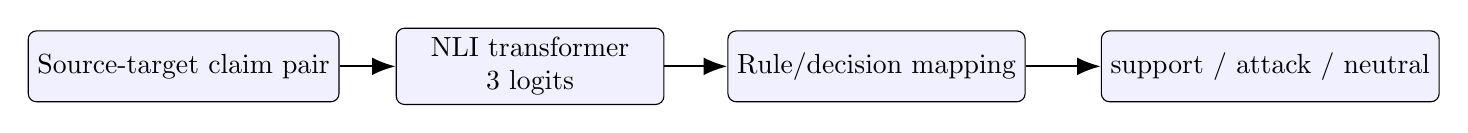
\begin{tikzpicture}[
  b/.style={draw, rounded corners=3pt, minimum width=3.4cm, minimum height=0.9cm, align=center, fill=blue!6},
  arrow/.style={-{Latex[length=3mm]}, thick}
]
\node[b] (pair) at (0,0) {Source-target claim pair};
\node[b] (nli) at (4.4,0) {NLI transformer\\3 logits};
\node[b] (rule) at (8.8,0) {Rule/decision mapping};
\node[b] (out) at (13.8,0) {support / attack / neutral};
\draw[arrow] (pair) -- (nli);
\draw[arrow] (nli) -- (rule);
\draw[arrow] (rule) -- (out);
\end{tikzpicture}
\caption{Architecture of the old DeBERTa rule/decision baseline.}
\end{figure}

\subsection{Old Stance Baseline}
\begin{figure}[htbp]
\centering
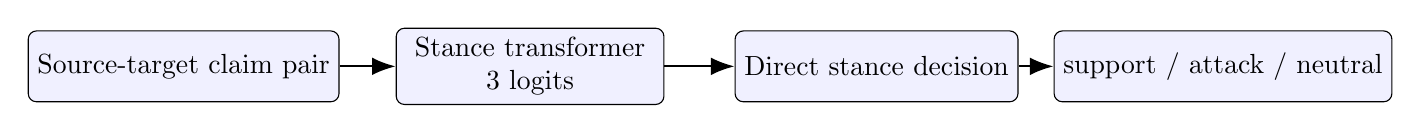
\begin{tikzpicture}[
  b/.style={draw, rounded corners=3pt, minimum width=3.4cm, minimum height=0.9cm, align=center, fill=blue!6},
  arrow/.style={-{Latex[length=3mm]}, thick}
]
\node[b] (pair) at (0,0) {Source-target claim pair};
\node[b] (stance) at (4.4,0) {Stance transformer\\3 logits};
\node[b] (decide) at (8.8,0) {Direct stance decision};
\node[b] (out) at (13.2,0) {support / attack / neutral};
\draw[arrow] (pair) -- (stance);
\draw[arrow] (stance) -- (decide);
\draw[arrow] (decide) -- (out);
\end{tikzpicture}
\caption{Architecture of the old stance-only baseline.}
\end{figure}

\subsection{Meta Logistic Regression Baseline}
\begin{figure}[htbp]
\centering
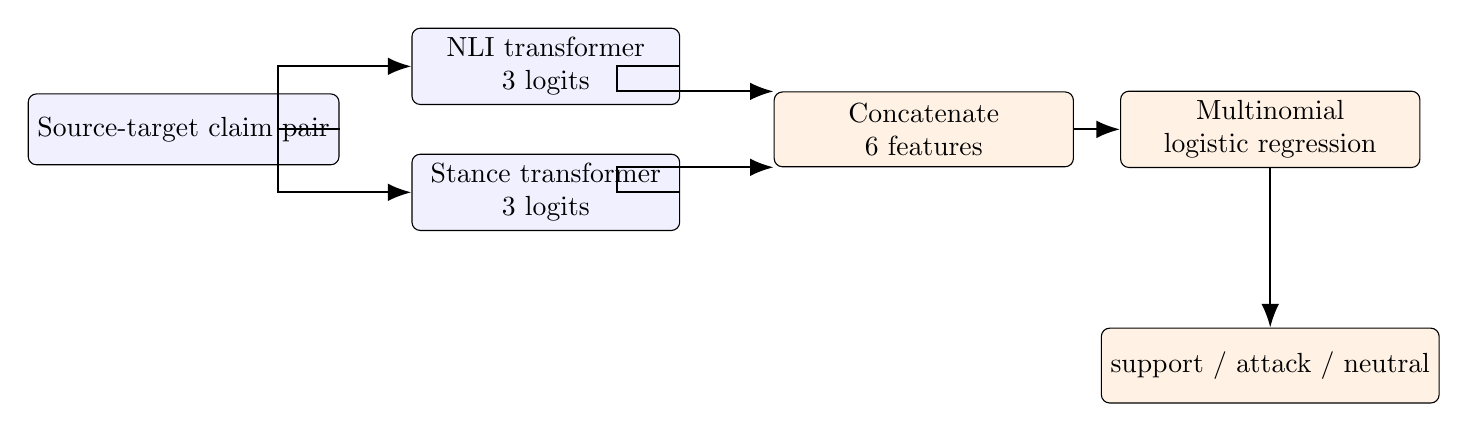
\begin{tikzpicture}[
  b/.style={draw, rounded corners=3pt, minimum width=3.4cm, minimum height=0.9cm, align=center, fill=blue!6},
  c/.style={draw, rounded corners=3pt, minimum width=3.8cm, minimum height=0.95cm, align=center, fill=orange!10},
  arrow/.style={-{Latex[length=3mm]}, thick}
]
\node[b] (pair) at (0,1.0) {Source-target claim pair};
\node[b] (nli) at (4.6,1.8) {NLI transformer\\3 logits};
\node[b] (stance) at (4.6,0.2) {Stance transformer\\3 logits};
\node[c] (concat) at (9.4,1.0) {Concatenate\\6 features};
\node[c] (lr) at (13.8,1.0) {Multinomial\\logistic regression};
\node[c] (out) at (13.8,-2.0) {support / attack / neutral};
\draw[arrow] (pair) -- ++(1.2,0) |- (nli.west);
\draw[arrow] (pair) -- ++(1.2,0) |- (stance.west);
\draw[arrow] (nli) -- ++(0.9,0) |- (concat.north west);
\draw[arrow] (stance) -- ++(0.9,0) |- (concat.south west);
\draw[arrow] (concat) -- (lr);
\draw[arrow] (lr) -- (out);
\end{tikzpicture}
\caption{Architecture of the DeBERTa + stance logistic-regression baseline.}
\end{figure}

\subsection{Graph-Statistic-Aware Model}
\begin{figure}[htbp]
\centering
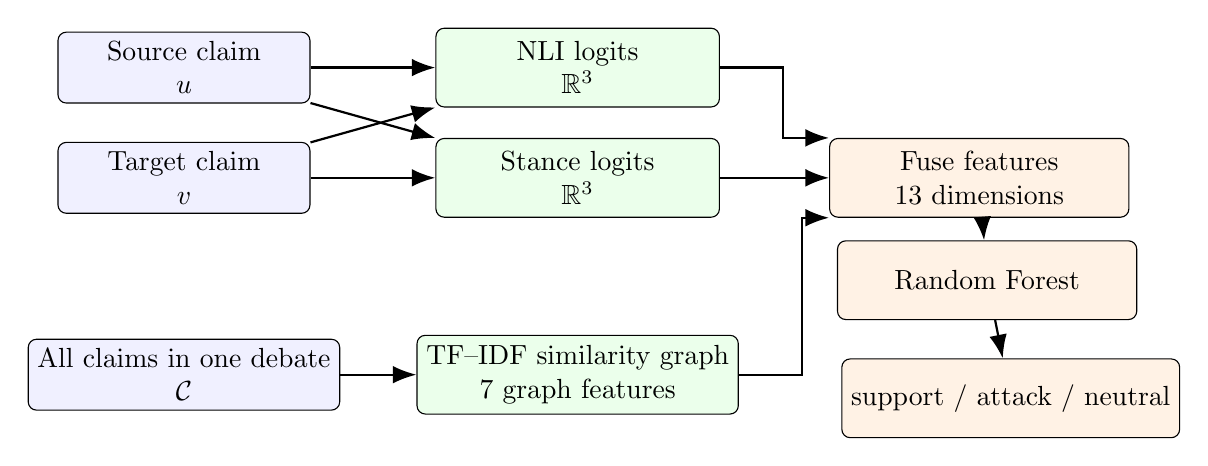
\begin{tikzpicture}[
  proc/.style={draw, rounded corners=3pt, minimum width=3.2cm, minimum height=0.9cm, align=center, fill=blue!6},
  feat/.style={draw, rounded corners=3pt, minimum width=3.6cm, minimum height=1.0cm, align=center, fill=green!8},
  cls/.style={draw, rounded corners=3pt, minimum width=3.8cm, minimum height=1.0cm, align=center, fill=orange!10},
  arrow/.style={-{Latex[length=3mm]}, thick}
]
\node[proc] (source) at (0,2.2) {Source claim\\\(u\)};
\node[proc] (target) at (0,0.8) {Target claim\\\(v\)};
\node[proc] (debate) at (0,-1.7) {All claims in one debate\\\(\mathcal{C}\)};
\node[feat] (nli) at (5.0,2.2) {NLI logits\\\(\mathbb{R}^3\)};
\node[feat] (stance) at (5.0,0.8) {Stance logits\\\(\mathbb{R}^3\)};
\node[feat] (graph) at (5.0,-1.7) {TF--IDF similarity graph\\7 graph features};
\node[cls] (concat) at (10.1,0.8) {Fuse features\\13 dimensions};
\node[cls] (forest) at (10.2,-0.5) {Random Forest};
\node[cls] (out) at (10.5,-2.0) {support / attack / neutral};
\draw[arrow] (source) -- (nli);
\draw[arrow] (target) -- (nli);
\draw[arrow] (source) -- (stance);
\draw[arrow] (target) -- (stance);
\draw[arrow] (debate) -- (graph);
\draw[arrow] (nli.east) -- ++(0.8,0) |- (concat.north west);
\draw[arrow] (stance.east) -- (concat.west);
\draw[arrow] (graph.east) -- ++(0.8,0) |- (concat.south west);
\draw[arrow] (concat) -- (forest);
\draw[arrow] (forest) -- (out);
\end{tikzpicture}
\caption{Architecture of the earlier graph-aware model.}
\end{figure}

The graph-statistic-aware model was the first serious attempt to move beyond purely pairwise classification while still
staying within a compact, interpretable tabular pipeline. The central intuition is that two claims should not be judged
only by what their texts say in isolation, but also by how they are positioned inside a debate-local semantic
neighborhood. Instead of introducing full graph message passing, the model builds a weighted similarity graph inside
each debate and summarizes the local geometry of a candidate pair with a small set of explicit graph statistics.

\paragraph{Debate-local similarity graph construction.}
Let the claims in a debate be \(\mathcal{C} = \{c_1,\dots,c_n\}\), and let \(\mathbf{t}_i\) be the debate-local
TF--IDF vector of claim \(c_i\). For any two claims \(c_i\) and \(c_j\), the semantic similarity score is:
\begin{equation}
s(c_i,c_j) = \cos(\mathbf{t}_i,\mathbf{t}_j)
\end{equation}

For each source claim \(c_i\), the model ranks all other claims by \(s(c_i,c_j)\), removes self-links, applies a
minimum similarity threshold \(\tau\), and retains only the top-\(k\) surviving neighbors:
\begin{equation}
N_k(c_i) = \operatorname{TopK}_{c_j \in \mathcal{C}\setminus \{c_i\}} \left\{ s(c_i,c_j) \; : \; s(c_i,c_j)\ge \tau \right\}
\end{equation}
In the saved benchmark configuration, \(k=8\) and \(\tau=0.15\). The result is a sparse debate-local semantic graph in
which edges do not represent gold argumentative relations directly; they represent local semantic affinity inside the
debate.

\paragraph{Seven graph-statistic features.}
For a directed candidate relation \((u,v)\), the graph-statistic-aware model appends the following seven features to
the six textual logits:
\begin{equation}
\mathbf{x}_{\mathrm{graph}}(u,v) =
\begin{bmatrix}
f_1 & f_2 & f_3 & f_4 & f_5 & f_6 & f_7
\end{bmatrix}
\in \mathbb{R}^{7}
\end{equation}

\textbf{Feature 1: Cosine similarity}
\begin{equation}
f_1(u,v) = \cos(\mathbf{t}_u,\mathbf{t}_v)
\end{equation}
This is the direct semantic-locality feature. It addresses the simplest failure mode of pairwise NLI and stance
predictions: two claims can be topically and lexically related even when the raw text-pair classifier is uncertain. If
\(u\) and \(v\) are very close in TF--IDF space inside the same debate, the edge is less likely to be a random neutral
pair. For example, if one claim says ``Executive orders allow immediate action'' and another says ``The president can
act faster than Congress,'' their local semantic closeness strongly suggests a meaningful discourse relation. This
feature turned out to be the strongest single graph-statistic feature in the ablation study.

\textbf{Feature 2: Normalized source degree}
\begin{equation}
f_2(u,v) = \frac{|N_k(u)|}{\max(1,k)}
\end{equation}
This feature estimates how many strong semantic neighbors the source claim has. It helps distinguish a highly connected
claim from a semantically isolated one. A source with many neighbors often corresponds to a broadly reusable or central
claim, whereas a low-degree source may be a narrow or idiosyncratic statement. The feature therefore acts as a local
context-strength prior.

\textbf{Feature 3: Normalized target degree}
\begin{equation}
f_3(u,v) = \frac{|N_k(v)|}{\max(1,k)}
\end{equation}
This is the target-side analogue of Feature 2. It captures whether the target is semantically central or peripheral in
the local debate geometry. This matters because a candidate edge pointing into a highly central target often behaves
differently from one pointing into a fringe claim.

\textbf{Feature 4: Target in source neighborhood}
\begin{equation}
f_4(u,v) = \mathbb{I}[v \in N_k(u)]
\end{equation}
This is a directed membership test. It answers the question: is the target one of the source claim's strongest local
semantic neighbors? This feature exists because rank and inclusion often matter more than raw similarity alone. A pair
may have moderate cosine similarity, but if the target still lands in the source's top semantic neighborhood, it is
more likely to be discourse-relevant than a pair with the same raw similarity but much lower relative rank.

\textbf{Feature 5: Source in target neighborhood}
\begin{equation}
f_5(u,v) = \mathbb{I}[u \in N_k(v)]
\end{equation}
This is the reverse directed membership test. Its purpose is to capture asymmetric locality. In semantic graphs, the
fact that \(v\) is one of \(u\)'s strongest neighbors does not guarantee the reverse, especially when one claim is much
broader than the other. This feature helps the model detect whether the pair is mutually local or only one-sidedly
local.

\textbf{Feature 6: Neighbor-set Jaccard overlap}
\begin{equation}
f_6(u,v) = \frac{|N_k(u) \cap N_k(v)|}{|N_k(u) \cup N_k(v)|}
\end{equation}
This feature measures whether the source and target live in the same local semantic region. It addresses a specific
problem that cosine similarity alone cannot solve: two claims may be directly similar, but the wider sets of claims
around them may still be very different. A large Jaccard overlap suggests that \(u\) and \(v\) participate in the same
subtopic cluster and therefore are more likely to bear a meaningful argumentative relation.

\textbf{Feature 7: Token-level Jaccard overlap}
\begin{equation}
f_7(u,v) = \frac{|T(u) \cap T(v)|}{|T(u) \cup T(v)|}
\end{equation}
where \(T(c)\) is the set of lowercased non-empty whitespace tokens in claim \(c\). This feature is a lightweight
surface-overlap signal. It helps when lexical reuse is informative even if the full TF--IDF geometry is noisy. For
example, if two claims both repeatedly use phrases such as ``executive order,'' ``Congress,'' or ``constitutional
basis,'' then token overlap can reinforce the conclusion that they belong to the same local argumentative region.

\paragraph{Fused graph-statistic-aware representation.}
The full input to the classifier is:
\begin{equation}
\mathbf{x}_{\mathrm{graphfull}}(u,v) =
\left[
\mathbf{x}_{\mathrm{NLI}} \; ; \; \mathbf{x}_{\mathrm{stance}} \; ; \; \mathbf{x}_{\mathrm{graph}}
\right]
\in \mathbb{R}^{13}
\end{equation}
The first six coordinates provide direct pairwise semantics, while the last seven coordinates summarize local graph
geometry. The graph-statistic-aware model therefore operationalizes the following hypothesis:
\begin{quote}
Two claims are easier to classify when the model knows not only what they say to each other, but also whether they are
neighbors in the same local semantic region of the debate.
\end{quote}

\paragraph{Classifier and training protocol.}
Given \(\mathbf{x}_{\mathrm{graphfull}}(u,v)\), the model predicts a class label with a Random Forest:
\begin{equation}
\hat{y}(u,v) = \arg\max_{c \in \{\texttt{support},\texttt{attack},\texttt{neutral}\}} P_{\mathrm{RF}}\!\left(c \mid \mathbf{x}_{\mathrm{graphfull}}(u,v)\right)
\end{equation}
The tree ensemble was chosen because it can model nonlinear interactions between textual and structural features
without requiring end-to-end neural retraining. In practice, this lets the model learn patterns such as:
\begin{itemize}[leftmargin=1.5em]
  \item high entailment plus high cosine similarity plus shared neighbors \(\Rightarrow\) likely support,
  \item moderate textual compatibility plus opposite stance evidence but strong local relevance \(\Rightarrow\) likely attack,
  \item weak textual evidence plus low graph locality \(\Rightarrow\) likely neutral.
\end{itemize}

\paragraph{What problem this model solves.}
The graph-statistic-aware design addresses a real weakness in the logistic-regression text-only fusion baseline. The
text-only model can tell whether two claims look compatible or contradictory, but it cannot tell whether they are
actually local to the same part of the debate. The seven graph-statistic features supply exactly that missing
information: not richer discourse ancestry yet, but at least a notion of local semantic placement, neighborhood
membership, and subtopic overlap.

\subsection{Proposed Ancestor-Context-Aware Model}
\begin{figure}[htbp]
\centering
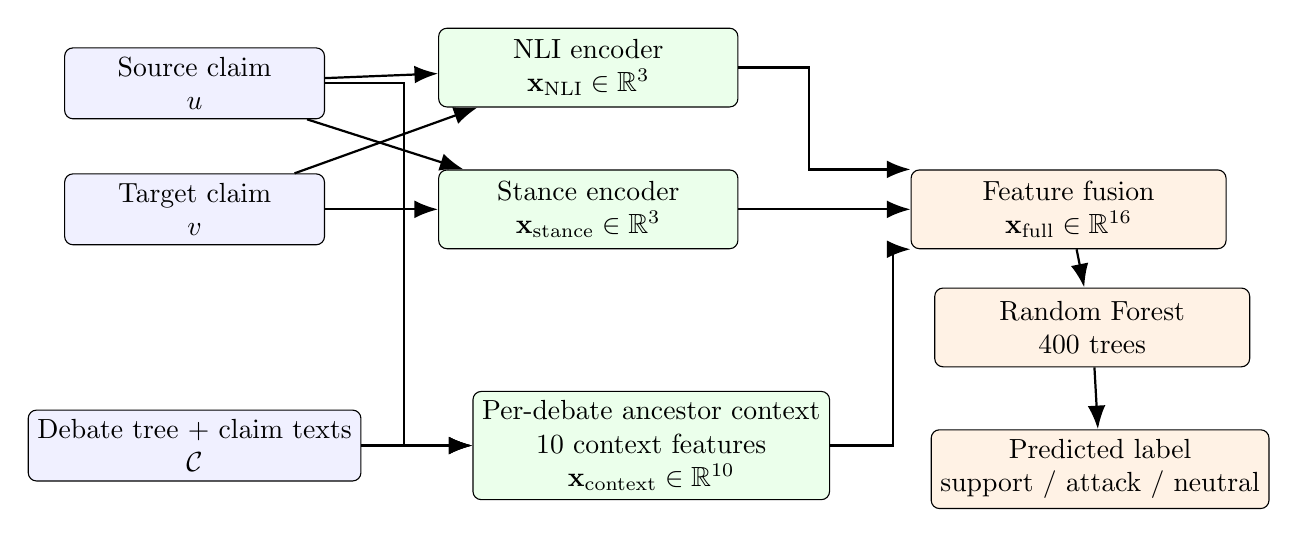
\begin{tikzpicture}[
  proc/.style={draw, rounded corners=3pt, minimum width=3.3cm, minimum height=0.9cm, align=center, fill=blue!6},
  feat/.style={draw, rounded corners=3pt, minimum width=3.8cm, minimum height=1.0cm, align=center, fill=green!8},
  cls/.style={draw, rounded corners=3pt, minimum width=4.0cm, minimum height=1.0cm, align=center, fill=orange!10},
  arrow/.style={-{Latex[length=3mm]}, thick}
]
\node[proc] (source) at (0,2.6) {Source claim\\\(u\)};
\node[proc] (target) at (0,1.0) {Target claim\\\(v\)};
\node[proc] (debate) at (0,-2.0) {Debate tree + claim texts\\\(\mathcal{C}\)};
\node[feat] (nli) at (5.0,2.8) {NLI encoder\\\(\mathbf{x}_{\mathrm{NLI}}\in\mathbb{R}^{3}\)};
\node[feat] (stance) at (5.0,1.0) {Stance encoder\\\(\mathbf{x}_{\mathrm{stance}}\in\mathbb{R}^{3}\)};
\node[feat] (context) at (5.8,-2.0) {Per-debate ancestor context\\10 context features\\\(\mathbf{x}_{\mathrm{context}}\in\mathbb{R}^{10}\)};
\node[cls] (concat) at (11.1,1.0) {Feature fusion\\\(\mathbf{x}_{\mathrm{full}}\in\mathbb{R}^{16}\)};
\node[cls] (forest) at (11.4,-0.5) {Random Forest\\400 trees};
\node[cls] (pred) at (11.5,-2.3) {Predicted label\\support / attack / neutral};
\draw[arrow] (source) -- (nli);
\draw[arrow] (target) -- (nli);
\draw[arrow] (source) -- (stance);
\draw[arrow] (target) -- (stance);
\draw[arrow] (debate) -- (context);
\draw[arrow] (source.east) -- ++(1.0,0) |- (context.west);
\draw[arrow] (target.east) -- ++(1.0,0) |- (context.west);
\draw[arrow] (nli.east) -- ++(0.9,0) |- (concat.north west);
\draw[arrow] (stance.east) -- (concat.west);
\draw[arrow] (context.east) -- ++(0.8,0) |- (concat.south west);
\draw[arrow] (concat) -- (forest);
\draw[arrow] (forest) -- (pred);
\end{tikzpicture}
\caption{Architecture of the proposed context-aware model.}
\end{figure}

\subsection{Classifier Choice}
The final classifier is a Random Forest with:
\begin{itemize}[leftmargin=1.5em]
  \item \texttt{n\_estimators = 400}
  \item \texttt{random\_state = 0}
  \item \texttt{n\_jobs = -1}
  \item \texttt{class\_weight = "balanced\_subsample"}
  \item \texttt{min\_samples\_leaf = 2}
\end{itemize}

Its prediction rule is:
\begin{equation}
\hat{\mathbf{p}}(\mathbf{x}_{\text{full}})
=
\frac{1}{M}\sum_{m=1}^{M} T_m(\mathbf{x}_{\text{full}}),
\qquad M=400
\end{equation}
\begin{equation}
\hat{y}
=
\arg\max_{c \in \{\texttt{support}, \texttt{attack}, \texttt{neutral}\}}
\hat{p}_c(\mathbf{x}_{\text{full}})
\end{equation}

\section{Results}
\subsection{Dedicated Analysis of the Graph-Statistic-Aware Model}
Before introducing the newer ancestor-context model as a successor, it is important to evaluate the graph-statistic-aware
model as a research contribution in its own right. On the saved benchmark split, the model reaches:
\begin{align}
\text{Accuracy}_{\mathrm{graph}} &= 0.8818 \\
\text{MacroF1}_{\mathrm{graph}} &= 0.8665 \\
\text{WeightedF1}_{\mathrm{graph}} &= 0.8811
\end{align}
These numbers are far above the direct DeBERTa baseline and the direct stance baseline, and they also substantially
improve over the text-only logistic-regression fusion baseline. This already shows that debate-local graph statistics
are not merely decorative features. They materially strengthen the classifier.

\subsection{Why the Graph-Statistic-Aware Model Works}
The graph-statistic-aware model helps because it solves a concrete ambiguity that pairwise text models often leave
unresolved. NLI and stance logits may indicate whether two claims are compatible, incompatible, or vague, but they do
not say whether the pair is actually discourse-local inside the debate. The graph-statistic-aware features add exactly
that missing locality signal.

In practical terms, the model succeeds when three conditions align:
\begin{enumerate}[label=\arabic*.]
  \item the pairwise encoders detect semantic compatibility or conflict,
  \item the similarity graph says the two claims lie in the same local semantic region,
  \item neighborhood overlap confirms that the pair is embedded in a common subtopic context rather than being a random topical coincidence.
\end{enumerate}
This is why the model performs so much better than the text-only fusion baseline: it can reject many irrelevant
cross-debate or cross-subtopic-looking pairs as neutral while still exploiting direct textual compatibility for support
and attack.

\subsection{Feature-Group Ablation of the Graph-Statistic-Aware Model}
The first ablation study isolates how much of the gain comes from the graph-statistic family as a whole.

\begin{center}
\begin{tabular}{lcccc}
\toprule
Subset & Features & Accuracy & Macro-F1 & Weighted-F1 \\
\midrule
\texttt{nli+stance+graph} & 13 & \textbf{0.8799} & \textbf{0.8650} & \textbf{0.8793} \\
\texttt{nli+graph} & 10 & 0.8780 & 0.8620 & 0.8774 \\
\texttt{nli+stance} & 6 & 0.6866 & 0.6710 & 0.6832 \\
\texttt{nli} & 3 & 0.6723 & 0.6607 & 0.6695 \\
\texttt{stance+graph} & 10 & 0.7173 & 0.6419 & 0.7122 \\
\texttt{graph} & 7 & 0.7095 & 0.6363 & 0.7069 \\
\texttt{stance} & 3 & 0.4441 & 0.3667 & 0.4232 \\
\bottomrule
\end{tabular}
\end{center}

This table makes three points clear. First, the graph-statistic family is genuinely useful on its own: the seven graph
features reach macro-F1 \(0.6363\), which is already much stronger than the direct stance-only baseline. Second, the
graph features combine especially well with NLI: \(\texttt{nli+graph}\) almost matches the full graph-statistic-aware
model, which means the NLI block and the graph-statistic block are highly complementary. Third, adding stance on top of
\(\texttt{nli+graph}\) yields only a small further increase, which suggests that the strongest interaction in the older
structured model is between semantic entailment/contradiction information and local graph geometry.

\subsection{Leave-One-Feature-Out Analysis of the Graph-Statistic-Aware Model}
The leave-one-feature-out study reveals how predictive value is distributed inside the seven-feature graph family.

\begin{center}
\begin{tabular}{lcccc}
\toprule
Dropped graph feature & Accuracy & Macro-F1 & Weighted-F1 & \(\Delta\) Macro-F1 \\
\midrule
\texttt{cosine\_similarity} & 0.8615 & 0.8445 & 0.8598 & \(-0.0212\) \\
\texttt{normalized\_source\_degree} & 0.8769 & 0.8618 & 0.8763 & \(-0.0039\) \\
\texttt{source\_in\_target} & 0.8776 & 0.8624 & 0.8771 & \(-0.0033\) \\
\texttt{target\_in\_source} & 0.8776 & 0.8624 & 0.8772 & \(-0.0033\) \\
\texttt{neighbor\_jaccard\_overlap} & 0.8795 & 0.8645 & 0.8790 & \(-0.0013\) \\
\texttt{normalized\_target\_degree} & 0.8806 & 0.8653 & 0.8801 & \(-0.0005\) \\
\texttt{token\_jaccard\_overlap} & 0.8810 & 0.8660 & 0.8806 & \(+0.0002\) \\
\bottomrule
\end{tabular}
\end{center}

This is one of the most important empirical findings in the whole project. The graph-statistic-aware model is clearly
helpful, but it is also clearly dominated by \texttt{cosine\_similarity}. Removing cosine similarity causes a macro-F1
drop of about \(0.0212\), which is dramatically larger than the drop caused by removing any other graph-statistic
feature. The degree, membership, and neighborhood-overlap features do contribute, but they behave more like secondary
refinement features than primary drivers.

This result should not be read as a failure. It is a strong scientific clue. It tells us that the old graph-aware
design is mainly valuable because it introduces a robust notion of debate-local semantic proximity. The limitation is
that it does not yet convert that locality information into a richer representation of upstream discourse structure.

\subsection{One-Feature-at-a-Time Analysis of the Graph-Statistic-Aware Model}
The one-feature-at-a-time study is also highly informative because it keeps the six textual logits fixed and allows
only one graph feature to be added at a time.

\begin{center}
\begin{tabular}{lccc}
\toprule
Kept graph feature & Accuracy & Macro-F1 & Weighted-F1 \\
\midrule
\texttt{cosine\_similarity} & \textbf{0.8803} & \textbf{0.8645} & \textbf{0.8795} \\
\texttt{token\_jaccard\_overlap} & 0.8202 & 0.8052 & 0.8191 \\
\texttt{target\_in\_source} & 0.8194 & 0.7994 & 0.8155 \\
\texttt{source\_in\_target} & 0.7980 & 0.7784 & 0.7941 \\
\texttt{neighbor\_jaccard\_overlap} & 0.7845 & 0.7657 & 0.7812 \\
\texttt{normalized\_target\_degree} & 0.7050 & 0.6883 & 0.7012 \\
\texttt{normalized\_source\_degree} & 0.6907 & 0.6747 & 0.6870 \\
\bottomrule
\end{tabular}
\end{center}

This study confirms the same hierarchy from a different angle. Cosine similarity is by far the strongest single
feature. The next best group consists of overlap and membership features, which still provide meaningful gains, but not
nearly at cosine's level. The degree features are useful only weakly in isolation, suggesting that degree behaves more
as contextual calibration than as a decisive signal by itself.

\subsection{Interpretation of the Graph-Statistic-Aware Model}
Taken together, the graph-statistic-aware results support the following interpretation.
\begin{enumerate}[label=\arabic*.]
  \item \textbf{The model is genuinely better than text-only fusion.} The gain over the logistic-regression baseline is too large to dismiss as noise. Local graph statistics clearly matter.
  \item \textbf{The dominant gain is semantic locality.} Most of the improvement comes from telling the classifier whether two claims live in the same semantic region of the debate.
  \item \textbf{The remaining graph statistics are supportive rather than dominant.} Degree, neighborhood membership, and Jaccard overlap refine the decision, but they do not drive it.
  \item \textbf{The model is graph-aware but not fully discourse-aware.} It knows where claims are in the local semantic graph, but it does not yet know how they relate to the upstream argument history that produced them.
\end{enumerate}

\subsection{Why the Graph-Statistic-Aware Model Remains Important}
Even though the ancestor-context model eventually outperforms it, the graph-statistic-aware model should still be
treated as a major methodological step rather than merely an intermediate baseline. It demonstrates that explicit
debate-local structure can materially improve stance detection even without a full neural graph model. It also provides
an interpretable bridge from text-only fusion to richer discourse-aware reasoning. In that sense, it plays the role of
an essential research stage: it establishes that structured context matters, and its own ablations reveal exactly which
parts of that context are still missing.

\subsection{Direct Feature-Family Comparison}
The clearest direct comparison between the older graph-statistic-aware model and the new graph-ancestor-context-aware model is to compare their full feature-family reference runs. These reference runs keep the same six textual features and differ only in the additional structured feature family that is appended.

\begin{center}
\begin{tabular}{lcccc}
\toprule
Model family & Text features & Extra features & Accuracy & Macro-F1 \\
\midrule
Graph-statistic-aware & 6 & 7 graph-statistic features & 0.8806 & 0.8658 \\
Graph-ancestor-context-aware & 6 & 10 ancestor-context features & \textbf{0.9441} & \textbf{0.9254} \\
\bottomrule
\end{tabular}
\end{center}

This comparison shows that the new gain is not simply coming from ``more features.'' The older model contributes local graph geometry, whereas the new model contributes upstream discourse context. The improvement is:
\begin{align*}
\Delta \text{Accuracy} &= 0.9441 - 0.8806 \approx 0.0634 \\
\Delta \text{Macro-F1} &= 0.9254 - 0.8658 \approx 0.0596
\end{align*}

\subsection{Overall Metrics}
\begin{center}
\begin{tabular}{lccc}
\toprule
Model & Accuracy & Macro-F1 & Weighted-F1 \\
\midrule
DeBERTa baseline & 0.5601 & 0.3907 & 0.4658 \\
Stance baseline & 0.3517 & 0.3104 & 0.3349 \\
DeBERTa + stance logistic regression & 0.6513 & 0.6557 & 0.6477 \\
Graph-aware model & 0.8818 & 0.8665 & 0.8811 \\
\textbf{Context-aware model} & \textbf{0.9433} & \textbf{0.9244} & \textbf{0.9433} \\
\bottomrule
\end{tabular}
\end{center}

\subsection{Metric Comparison Bar Charts}
\begin{figure}[htbp]
\centering
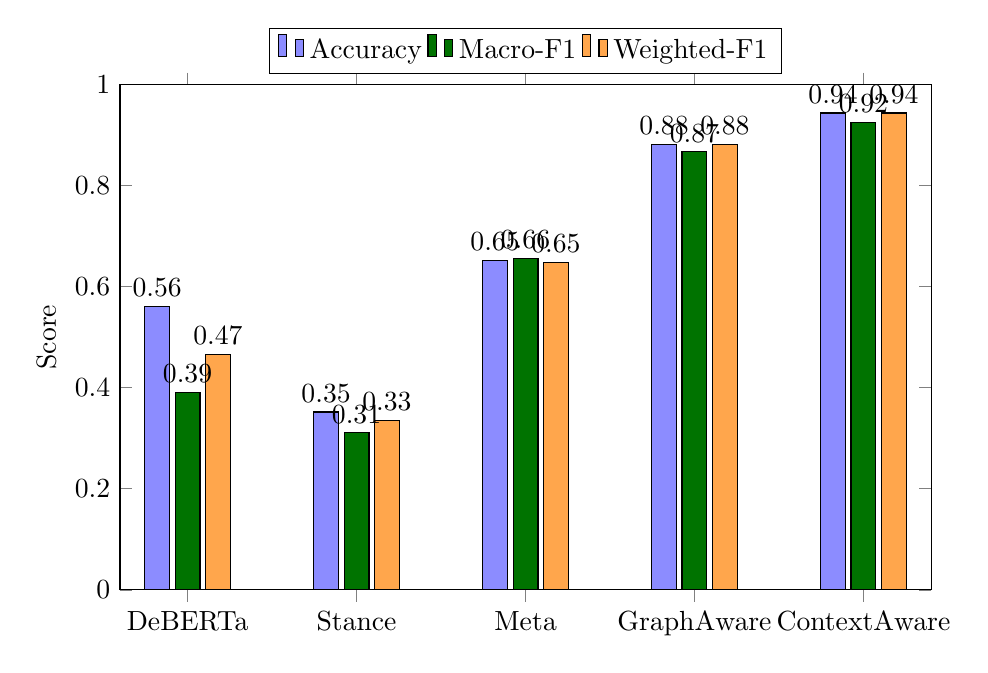
\begin{tikzpicture}
\begin{axis}[
    ybar,
    bar width=9pt,
    width=0.98\textwidth,
    height=8cm,
    ymin=0,
    ymax=1.0,
    ylabel={Score},
    symbolic x coords={DeBERTa,Stance,Meta,GraphAware,ContextAware},
    xtick=data,
    legend style={at={(0.5,1.02)}, anchor=south, legend columns=3},
    nodes near coords,
    nodes near coords align={vertical},
    enlarge x limits=0.10
]
\addplot[fill=blue!45] coordinates {
  (DeBERTa,0.5601)
  (Stance,0.3517)
  (Meta,0.6513)
  (GraphAware,0.8818)
  (ContextAware,0.9433)
};
\addplot[fill=green!45!black] coordinates {
  (DeBERTa,0.3907)
  (Stance,0.3104)
  (Meta,0.6557)
  (GraphAware,0.8665)
  (ContextAware,0.9244)
};
\addplot[fill=orange!70] coordinates {
  (DeBERTa,0.4658)
  (Stance,0.3349)
  (Meta,0.6477)
  (GraphAware,0.8811)
  (ContextAware,0.9433)
};
\legend{Accuracy, Macro-F1, Weighted-F1}
\end{axis}
\end{tikzpicture}
\caption{Comparison of all evaluated models across the three primary aggregate metrics.}
\end{figure}

\subsection{Per-Class Scores}
\begin{center}
\begin{tabular}{llccc}
\toprule
Model & Class & Precision & Recall & F1 \\
\midrule
\multirow{3}{*}{DeBERTa}
  & Support & 0.8182 & 0.1081 & 0.1910 \\
  & Attack  & 0.8722 & 0.1742 & 0.2904 \\
  & Neutral & 0.5338 & 0.9790 & 0.6909 \\
\midrule
\multirow{3}{*}{Stance}
  & Support & 0.2607 & 0.7162 & 0.3822 \\
  & Attack  & 0.2844 & 0.0931 & 0.1403 \\
  & Neutral & 0.6461 & 0.2988 & 0.4086 \\
\midrule
\multirow{3}{*}{Meta}
  & Support & 0.5726 & 0.7102 & 0.6340 \\
  & Attack  & 0.6257 & 0.8183 & 0.7092 \\
  & Neutral & 0.7415 & 0.5383 & 0.6237 \\
\midrule
\multirow{3}{*}{Graph-aware}
  & Support & 0.8485 & 0.8243 & 0.8363 \\
  & Attack  & 0.8525 & 0.8243 & 0.8382 \\
  & Neutral & 0.9111 & 0.9392 & 0.9250 \\
\midrule
\multirow{3}{*}{\textbf{Graph-Ancestor-Context-aware}}
  & Support & \textbf{0.8884} & \textbf{0.8844} & \textbf{0.8864} \\
  & Attack  & \textbf{0.8849} & \textbf{0.8889} & \textbf{0.8869} \\
  & Neutral & \textbf{1.0000} & \textbf{1.0000} & \textbf{1.0000} \\
\bottomrule
\end{tabular}
\end{center}

\subsection{Confusion Matrices}
Using label order \([\texttt{support}, \texttt{attack}, \texttt{neutral}]\):

\paragraph{DeBERTa baseline}
\[
\begin{bmatrix}
72 & 2 & 592 \\
3 & 116 & 547 \\
13 & 15 & 1304
\end{bmatrix}
\]

\paragraph{Stance baseline}
\[
\begin{bmatrix}
477 & 74 & 115 \\
501 & 62 & 103 \\
852 & 82 & 398
\end{bmatrix}
\]

\paragraph{Meta baseline}
\[
\begin{bmatrix}
473 & 39 & 154 \\
25 & 545 & 96 \\
328 & 287 & 717
\end{bmatrix}
\]

\paragraph{Graph-aware model}
\[
\begin{bmatrix}
549 & 56 & 61 \\
56 & 549 & 61 \\
42 & 39 & 1251
\end{bmatrix}
\]

\paragraph{Context-aware model}
\[
\begin{bmatrix}
589 & 77 & 0 \\
74 & 592 & 0 \\
0 & 0 & 1332
\end{bmatrix}
\]

\subsection{Confusion Matrix Figures for All Methods}
\begin{figure}[H]
\centering
\begin{minipage}{0.48\textwidth}
\centering
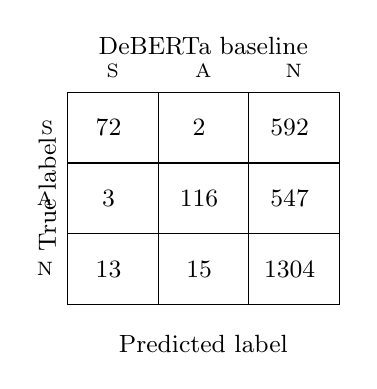
\begin{tikzpicture}[scale=0.60]
\matrix[matrix of nodes,
nodes={draw, minimum width=1.15cm, minimum height=0.9cm, align=center, font=\small},
row sep=-\pgflinewidth, column sep=-\pgflinewidth] (m) {
72 & 2 & 592 \\
3 & 116 & 547 \\
13 & 15 & 1304 \\
};
\node[above=0.35cm of m-1-2] {\small DeBERTa baseline};
\node[left=0.25cm of m-1-1, rotate=90] {\small True label};
\node[below=0.25cm of m-3-2] {\small Predicted label};
\node[above=0.05cm of m-1-1] {\scriptsize S};
\node[above=0.05cm of m-1-2] {\scriptsize A};
\node[above=0.05cm of m-1-3] {\scriptsize N};
\node[left=0.05cm of m-1-1] {\scriptsize S};
\node[left=0.05cm of m-2-1] {\scriptsize A};
\node[left=0.05cm of m-3-1] {\scriptsize N};
\end{tikzpicture}
\end{minipage}
\hfill
\begin{minipage}{0.48\textwidth}
\centering
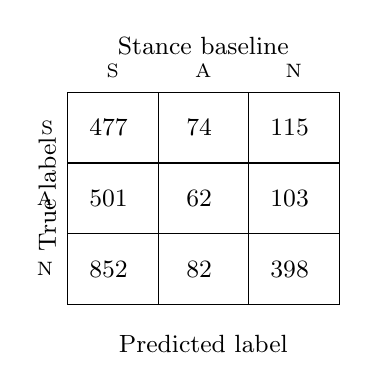
\begin{tikzpicture}[scale=0.60]
\matrix[matrix of nodes,
nodes={draw, minimum width=1.15cm, minimum height=0.9cm, align=center, font=\small},
row sep=-\pgflinewidth, column sep=-\pgflinewidth] (m) {
477 & 74 & 115 \\
501 & 62 & 103 \\
852 & 82 & 398 \\
};
\node[above=0.35cm of m-1-2] {\small Stance baseline};
\node[left=0.25cm of m-1-1, rotate=90] {\small True label};
\node[below=0.25cm of m-3-2] {\small Predicted label};
\node[above=0.05cm of m-1-1] {\scriptsize S};
\node[above=0.05cm of m-1-2] {\scriptsize A};
\node[above=0.05cm of m-1-3] {\scriptsize N};
\node[left=0.05cm of m-1-1] {\scriptsize S};
\node[left=0.05cm of m-2-1] {\scriptsize A};
\node[left=0.05cm of m-3-1] {\scriptsize N};
\end{tikzpicture}
\end{minipage}

\vspace{0.55cm}

\begin{minipage}{0.48\textwidth}
\centering
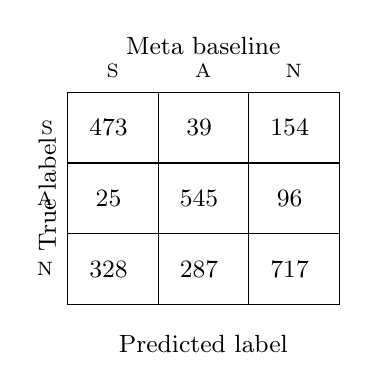
\begin{tikzpicture}[scale=0.60]
\matrix[matrix of nodes,
nodes={draw, minimum width=1.15cm, minimum height=0.9cm, align=center, font=\small},
row sep=-\pgflinewidth, column sep=-\pgflinewidth] (m) {
473 & 39 & 154 \\
25 & 545 & 96 \\
328 & 287 & 717 \\
};
\node[above=0.35cm of m-1-2] {\small Meta baseline};
\node[left=0.25cm of m-1-1, rotate=90] {\small True label};
\node[below=0.25cm of m-3-2] {\small Predicted label};
\node[above=0.05cm of m-1-1] {\scriptsize S};
\node[above=0.05cm of m-1-2] {\scriptsize A};
\node[above=0.05cm of m-1-3] {\scriptsize N};
\node[left=0.05cm of m-1-1] {\scriptsize S};
\node[left=0.05cm of m-2-1] {\scriptsize A};
\node[left=0.05cm of m-3-1] {\scriptsize N};
\end{tikzpicture}
\end{minipage}
\hfill
\begin{minipage}{0.48\textwidth}
\centering
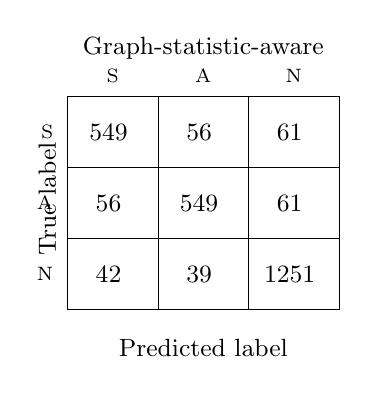
\begin{tikzpicture}[scale=0.60]
\matrix[matrix of nodes,
nodes={draw, minimum width=1.15cm, minimum height=0.9cm, align=center, font=\small},
row sep=-\pgflinewidth, column sep=-\pgflinewidth] (m) {
549 & 56 & 61 \\
56 & 549 & 61 \\
42 & 39 & 1251 \\
};
\node[above=0.35cm of m-1-2] {\small Graph-statistic-aware};
\node[left=0.25cm of m-1-1, rotate=90] {\small True label};
\node[below=0.25cm of m-3-2] {\small Predicted label};
\node[above=0.05cm of m-1-1] {\scriptsize S};
\node[above=0.05cm of m-1-2] {\scriptsize A};
\node[above=0.05cm of m-1-3] {\scriptsize N};
\node[left=0.05cm of m-1-1] {\scriptsize S};
\node[left=0.05cm of m-2-1] {\scriptsize A};
\node[left=0.05cm of m-3-1] {\scriptsize N};
\end{tikzpicture}
\end{minipage}
\caption{Confusion matrices for the four earlier methods.}
\end{figure}

\subsection{Graph-Ancestor-Context-Aware Confusion Matrix}
\begin{figure}[H]
\centering
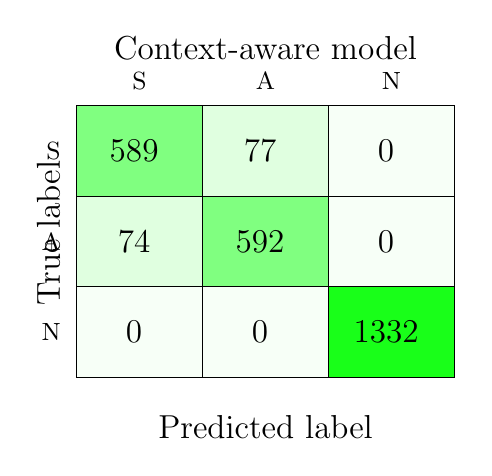
\begin{tikzpicture}[scale=0.82]
\matrix[matrix of nodes,
nodes={draw, minimum width=1.6cm, minimum height=1.15cm, align=center, font=\large},
row sep=-\pgflinewidth, column sep=-\pgflinewidth] (m) {
|[fill=green!50]|589 & |[fill=green!12]|77 & |[fill=green!3]|0 \\
|[fill=green!12]|74 & |[fill=green!50]|592 & |[fill=green!3]|0 \\
|[fill=green!3]|0 & |[fill=green!3]|0 & |[fill=green!90]|1332 \\
};
\node[above=0.45cm of m-1-2] {\large Context-aware model};
\node[left=0.35cm of m-1-1, rotate=90] {\large True label};
\node[below=0.35cm of m-3-2] {\large Predicted label};
\node[above=0.07cm of m-1-1] {\small S};
\node[above=0.07cm of m-1-2] {\small A};
\node[above=0.07cm of m-1-3] {\small N};
\node[left=0.07cm of m-1-1] {\small S};
\node[left=0.07cm of m-2-1] {\small A};
\node[left=0.07cm of m-3-1] {\small N};
\end{tikzpicture}
\caption{Confusion matrix of the proposed graph-ancestor-context-aware model. The neutral class is perfectly separated on this saved benchmark split, while support and attack remain the main source of residual confusion.}
\end{figure}

\section{Interpretation of Results}
\subsection{Main Quantitative Findings}
The new context-aware model achieves:
\begin{align*}
\text{Accuracy} &= 0.9433 \\
\text{Macro-F1} &= 0.9244 \\
\text{Weighted-F1} &= 0.9433
\end{align*}

Compared to the earlier graph-aware model:
\begin{align*}
\Delta \text{Accuracy} &= 0.9433 - 0.8818 \approx 0.0615 \\
\Delta \text{Macro-F1} &= 0.9244 - 0.8665 \approx 0.0579
\end{align*}

Compared to the logistic-regression meta baseline:
\begin{align*}
\Delta \text{Accuracy} &= 0.9433 - 0.6513 \approx 0.2920 \\
\Delta \text{Macro-F1} &= 0.9244 - 0.6557 \approx 0.2687
\end{align*}

\subsection{Understanding the Graph-Statistic-Aware Error Profile}
The graph-statistic-aware confusion matrix is:
\[
\begin{bmatrix}
549 & 56 & 61 \\
56 & 549 & 61 \\
42 & 39 & 1251
\end{bmatrix}
\]
This matrix is important because it explains both the strength and the limitation of the older structured model.

The strength is immediately visible in the neutral row. The model correctly classifies \(1251\) of \(1332\) neutral
examples, which means that local semantic geometry is already quite effective at rejecting many sampled non-edges. This
is exactly what the graph-statistic-aware design was meant to improve over text-only fusion.

The limitation is visible in the symmetric support--attack confusion. The model makes \(56\) support\(\rightarrow\)attack
errors and \(56\) attack\(\rightarrow\)support errors, with another \(61\) support\(\rightarrow\)neutral and \(61\)
attack\(\rightarrow\)neutral errors. This pattern suggests that the model is good at deciding whether a pair is
meaningful, but still less certain about the exact polarity of that meaning. In other words, the older structured model
captures local relevance better than it captures upstream argumentative orientation.

This interpretation is fully consistent with the feature ablations. A model dominated by cosine similarity, neighbor
membership, and overlap should be expected to excel at answering:
\begin{quote}
Do these two claims belong to the same local semantic region?
\end{quote}
but not necessarily:
\begin{quote}
How does the source claim position itself relative to the target claim's argument history?
\end{quote}
That second question is exactly what motivated the later ancestor-context design.

\subsection{Weaknesses Addressed by the Graph-Ancestor-Context-Aware Design}
The older graph-statistic-aware model fixed an important limitation of purely pairwise classification, but its ablations exposed three weaknesses.

\begin{enumerate}[label=\arabic*.]
  \item \textbf{Over-reliance on direct pair similarity.} In the graph-statistic-aware ablation, dropping \texttt{cosine\_similarity} reduces macro-F1 by about \(0.0212\), far more than dropping any other graph feature. This indicates that the older model was dominated by one direct semantic-locality signal.
  \item \textbf{Weak access to upstream discourse.} Degree, membership, and Jaccard overlap explain local graph geometry, but they do not explain how a claim emerges from its parent and ancestor chain.
  \item \textbf{Limited cross-context reasoning.} The older model can tell that two claims are locally close, but it cannot directly test whether one claim agrees with the other claim's upstream discourse history.
\end{enumerate}

The new graph-ancestor-context-aware model is designed to address exactly these weaknesses by encoding:
\begin{itemize}[leftmargin=1.5em]
  \item depth and depth gap,
  \item amount of upstream context available to each claim,
  \item claim-to-own-context similarity,
  \item claim-to-other-context similarity,
  \item context-to-context similarity.
\end{itemize}

\subsection{Why the Context-Aware Model Helps}
The results strongly support the hypothesis that ancestor context carries richer information than shallow local graph statistics alone.
\begin{enumerate}[label=\arabic*.]
  \item \textbf{Upstream discourse context reduces ambiguity.} A source-target pair becomes easier to classify when the system knows how each claim aligns with its own ancestor chain and with the other claim's ancestor context.
  \item \textbf{Neutral separation becomes dramatically cleaner.} The context-aware model achieves perfect precision and recall on the neutral class for this saved benchmark split.
  \item \textbf{Support and attack remain balanced.} Support and attack are both near \(0.886\) F1, which is much healthier than the strong class biases seen in the older baselines.
  \item \textbf{Cross-context similarity appears to matter more than flat overlap.} The older graph-aware model was dominated by direct cosine similarity, whereas the new model uses claim-to-context and context-to-context similarity and improves substantially.
\end{enumerate}

\subsection{Feature-Group Ablation of the Graph-Ancestor-Context-Aware Model}
The feature-group ablation for the new model is:

\begin{center}
\begin{tabular}{lcccc}
\toprule
Subset & Features & Accuracy & Macro-F1 & Weighted-F1 \\
\midrule
\texttt{nli+stance+context} & 16 & \textbf{0.9441} & \textbf{0.9254} & \textbf{0.9441} \\
\texttt{nli+context} & 13 & 0.9414 & 0.9219 & 0.9414 \\
\texttt{stance+context} & 13 & 0.7898 & 0.7172 & 0.7879 \\
\texttt{context} & 10 & 0.7815 & 0.7087 & 0.7815 \\
\texttt{nli+stance} & 6 & 0.6866 & 0.6710 & 0.6832 \\
\texttt{nli} & 3 & 0.6723 & 0.6607 & 0.6695 \\
\texttt{stance} & 3 & 0.4441 & 0.3667 & 0.4232 \\
\bottomrule
\end{tabular}
\end{center}

This ablation makes two points very clear:
\begin{enumerate}[label=\arabic*.]
  \item The context feature family is genuinely strong on its own. The \texttt{context}-only subset reaches macro-F1 \(0.7087\), comfortably above the stance-only baseline and above pure NLI.
  \item The context family is especially complementary to NLI. The \texttt{nli+context} subset already reaches macro-F1 \(0.9219\), which is nearly as strong as the full model.
\end{enumerate}

\subsection{Direct Graph-Statistic-Aware vs Graph-Ancestor-Context-Aware Feature Comparison}
The two structured feature families can also be compared directly through their family-level ablations.

\begin{center}
\begin{tabular}{lccc}
\toprule
Feature family & Feature count & Standalone Macro-F1 & Best paired Macro-F1 \\
\midrule
Graph-statistic-aware & 7 & 0.6363 & 0.8620 (\texttt{nli+graph}) \\
Graph-ancestor-context-aware & 10 & \textbf{0.7087} & \textbf{0.9219} (\texttt{nli+context}) \\
\bottomrule
\end{tabular}
\end{center}

This is a strong result. The newer feature family is not just better in the full model; it is also intrinsically more informative both as a standalone structured signal and as an add-on to the strongest pairwise text block.

\subsection{Leave-One-Feature-Out Ablation of the Graph-Ancestor-Context-Aware Model}
The leave-one-feature-out context ablation reveals which new features matter most.

\begin{center}
\begin{tabular}{lcc}
\toprule
Dropped context feature & Macro-F1 & \(\Delta\) Macro-F1 vs full \\
\midrule
\texttt{target\_to\_source\_ancestor\_context} & 0.9215 & \(-0.0040\) \\
\texttt{normalized\_target\_ancestor\_count} & 0.9229 & \(-0.0025\) \\
\texttt{normalized\_source\_depth} & 0.9239 & \(-0.0015\) \\
\texttt{target\_to\_own\_ancestor\_context} & 0.9244 & \(-0.0010\) \\
\texttt{normalized\_source\_ancestor\_count} & 0.9254 & \(+0.0000\) \\
\texttt{ancestor\_context\_to\_ancestor\_context} & 0.9254 & \(+0.0000\) \\
\texttt{source\_to\_own\_ancestor\_context} & 0.9259 & \(+0.0005\) \\
\texttt{normalized\_target\_depth} & 0.9259 & \(+0.0005\) \\
\texttt{normalized\_depth\_gap} & 0.9269 & \(+0.0015\) \\
\texttt{source\_to\_target\_ancestor\_context} & \textbf{0.9284} & \textbf{\(+0.0030\)} \\
\bottomrule
\end{tabular}
\end{center}

The most damaging feature to remove is \texttt{target\_to\_source\_ancestor\_context}. This is a particularly meaningful result because it directly supports the core thesis of the model: cross-context interaction is more important than flat overlap.

\subsection{One-Feature-at-a-Time Context Ablation}
The one-feature-at-a-time study with \(\texttt{nli}+\texttt{stance}+1\) context feature gives an especially interpretable result.

\begin{center}
\begin{tabular}{lcc}
\toprule
Kept context feature & Macro-F1 & Accuracy \\
\midrule
\texttt{target\_to\_source\_ancestor\_context} & \textbf{0.9299} & \textbf{0.9474} \\
\texttt{ancestor\_context\_to\_ancestor\_context} & 0.9204 & 0.9373 \\
\texttt{normalized\_depth\_gap} & 0.7741 & 0.7815 \\
\texttt{normalized\_target\_depth} & 0.7627 & 0.7691 \\
\texttt{normalized\_target\_ancestor\_count} & 0.7627 & 0.7691 \\
\texttt{source\_to\_target\_ancestor\_context} & 0.7391 & 0.7541 \\
\texttt{source\_to\_own\_ancestor\_context} & 0.6750 & 0.6903 \\
\texttt{target\_to\_own\_ancestor\_context} & 0.6731 & 0.6884 \\
\texttt{normalized\_source\_depth} & 0.6692 & 0.6858 \\
\texttt{normalized\_source\_ancestor\_count} & 0.6692 & 0.6858 \\
\bottomrule
\end{tabular}
\end{center}

This result is striking: one carefully chosen ancestor-context feature, \texttt{target\_to\_source\_ancestor\_context}, already outperforms the earlier graph-statistic-aware model. That strongly suggests that the new model's gains are being driven by a more relevant representation of discourse context rather than by a larger feature budget alone.

\subsection{Direct Ablation Comparison Between the Two Structured Models}
The ablation evidence becomes even clearer when the older graph-statistic-aware model and the newer graph-ancestor-context-aware model are compared side by side.

\paragraph{1. Feature-group comparison.}
Table~\ref{tab:structured_ablation_family_compare} compares the three most interpretable checkpoints for the two structured feature families.

\begin{table}[H]
\centering
\caption{Feature-group ablation comparison between the graph-statistic-aware and graph-ancestor-context-aware families. Values are macro-F1.}
\label{tab:structured_ablation_family_compare}
\begin{tabular}{lccc}
\toprule
Structured family & Structured only & NLI + structured & NLI + stance + structured \\
\midrule
Graph-statistic-aware & 0.6363 & 0.8620 & 0.8650 \\
Graph-ancestor-context-aware & \textbf{0.7087} & \textbf{0.9219} & \textbf{0.9254} \\
\bottomrule
\end{tabular}
\end{table}

This comparison shows that the newer context family is stronger in all three settings. It is better as a standalone structured signal, better as a complement to NLI, and better in the fully fused model. That pattern matters because it shows that the new gains are not coming from a single lucky interaction with one text block; they reflect a genuinely more informative representation of discourse structure.

\paragraph{2. Leave-one-feature-out comparison.}
The leave-one-feature-out results expose how concentrated or distributed the predictive value is inside each structured family.

\begin{table}[H]
\centering
\caption{Most damaging leave-one-feature-out removal in each structured family.}
\label{tab:structured_ablation_loo_compare}
\begin{tabular}{lcc}
\toprule
Structured family & Most damaging dropped feature & \(\Delta\) macro-F1 \\
\midrule
Graph-statistic-aware & \texttt{cosine\_similarity} & \(-0.0212\) \\
Graph-ancestor-context-aware & \texttt{target\_to\_source\_ancestor\_context} & \(-0.0040\) \\
\bottomrule
\end{tabular}
\end{table}

The older graph-statistic-aware model is dominated by one feature. Removing \texttt{cosine\_similarity} reduces macro-F1 by about \(0.0212\), whereas removing most other graph features changes macro-F1 by only a few thousandths. This means that the earlier model behaves largely like a pairwise classifier plus one strong similarity cue.

The newer graph-ancestor-context-aware model is more distributed. Its strongest negative drop comes from removing \texttt{target\_to\_source\_ancestor\_context}, which lowers macro-F1 by about \(0.0040\). This is still meaningful, but much smaller than the dominance gap seen for cosine similarity in the older model. In other words, the newer model is less fragile and less dependent on a single scalar proximity feature.

\paragraph{3. One-feature-at-a-time comparison.}
The one-feature-at-a-time setting gives the cleanest direct comparison because it holds the six textual features fixed and asks which single structured feature contributes the most additional value.

\begin{table}[H]
\centering
\caption{Best single structured feature on top of NLI + stance.}
\label{tab:structured_ablation_single_compare}
\begin{tabular}{lccc}
\toprule
Structured family & Best single feature & Macro-F1 & Accuracy \\
\midrule
Graph-statistic-aware & \texttt{cosine\_similarity} & 0.8645 & 0.8803 \\
Graph-ancestor-context-aware & \textbf{\texttt{target\_to\_source\_ancestor\_context}} & \textbf{0.9299} & \textbf{0.9474} \\
\bottomrule
\end{tabular}
\end{table}

This is the strongest direct comparison in the paper. It shows that one carefully chosen ancestor-context feature is more informative than the best single graph-statistic feature, and in fact stronger than the entire earlier graph-statistic-aware full model.

\paragraph{4. Interpretation.}
The older graph-statistic-aware model mainly answers:
\begin{quote}
Are these two claims locally close in the semantic graph?
\end{quote}

The newer graph-ancestor-context-aware model answers a richer question:
\begin{quote}
How does each claim relate to its own upstream argument history, and how does each claim relate to the other claim's upstream history?
\end{quote}

That difference explains why the newer feature family produces stronger ablation results. It is not just encoding that two claims are similar. It is encoding how they are situated inside the argument tree that generated them.

\paragraph{5. Weaknesses addressed.}
The direct ablation comparison makes it possible to state more precisely which weaknesses of the older graph-statistic-aware design are being addressed.
\begin{enumerate}[label=\arabic*.]
  \item \textbf{Over-reliance on semantic proximity.} The older model leans heavily on \texttt{cosine\_similarity}, which means that much of its improvement can be explained by a single local-neighborhood cue. The newer model spreads predictive value across several ancestor-context features instead of relying on one dominant scalar.
  \item \textbf{Weak access to upstream discourse.} Degree, membership, and Jaccard overlap describe graph shape, but they do not explicitly represent how a claim is supported, challenged, or contextualized by the argument chain above it. The new feature family directly encodes that upstream context.
  \item \textbf{Limited cross-context reasoning.} The older family does not directly test whether a source claim is coherent with the target claim's ancestor history, or vice versa. The strongest new feature, \texttt{target\_to\_source\_ancestor\_context}, addresses exactly this missing interaction.
\end{enumerate}

\subsection{Connection to GraphNLI}
The new model is not a direct implementation of GraphNLI, but it is strongly inspired by its core idea. GraphNLI argues that polarity prediction improves when the model incorporates wider discussion context, especially through root-seeking or ancestor-oriented context. The present model translates that intuition into a feature-based design:
\begin{itemize}[leftmargin=1.5em]
  \item GraphNLI uses graph walks and contextual embeddings,
  \item the present model uses explicit ancestor chains and weighted ancestor-context TF--IDF embeddings,
  \item both approaches emphasize upstream discourse context rather than isolated pairwise semantics.
\end{itemize}

\section{Limitations and Caveats}
\begin{itemize}[leftmargin=1.5em]
  \item The saved benchmark is still small: only eight debates are used.
  \item The ancestor-context branch is TF--IDF based rather than end-to-end neural.
  \item Neutral performance still depends on the non-edge sampling policy.
  \item The model is context-aware, but not yet a full graph neural architecture.
  \item Several leave-one-out context ablations slightly outperform the nominal full model, which suggests that the current 10-feature context set is already strong but not yet perfectly minimal.
\end{itemize}

\section{Next Steps}
The most important next experiments are:
\begin{enumerate}[label=\arabic*.]
  \item run the context-aware benchmark on more debates and multiple seeds,
  \item perform dedicated ablation studies on the ten context features,
  \item compare context-aware features directly against the earlier graph-aware features,
  \item test hybrid models that combine the 7 graph-aware features and the 10 context-aware features,
  \item replace TF--IDF ancestor embeddings with transformer-based ancestor-context embeddings.
\end{enumerate}

\section{Conclusion}
The context-aware stance detection model introduced here is a stronger successor to the earlier graph-aware design. It preserves the successful pairwise transformer backbone, but replaces shallow neighborhood statistics with a richer upstream discourse-context representation. On the current saved Syncialo benchmark split, it substantially outperforms the old DeBERTa baseline, the old stance baseline, the logistic-regression fusion baseline, and the earlier graph-aware model.

Its main contribution is not only higher accuracy, but a more discourse-faithful representation of debate structure. The model does not merely ask whether two claims are similar; it asks whether each claim is coherent with the argument history leading up to it, and whether those histories align with one another.

\end{document}
